\subsubsection{The solution of Data Hazards}

The following techniques don't solve the problem completely, but they do solve it partially. So they find a perfect balance between the ideal speedup and a situation where the hazard is total.

\highspace
The solution can be applied on runtime (hardware techniques) or on compilation (static-time techniques):
\begin{itemize}
    \item \textbf{Compilation Techniques} (static-time techniques):
    \begin{itemize}
        \item The \indexdefinition{insertion of \texttt{nop}} is a simple (logical) solution where we \textbf{insert a \texttt{nop} operator between dependent statements} to ensure correct operation.

        See the \example{example} on page \pageref{example: insertion of nop}.


        \item The \indexdefinition{instructions scheduling} is a technique used by the compiler to prevent correlating instructions from being too close together. It tries to \textbf{reorder instructions} by inserting independent instructions between correlating instructions. \textbf{If the compiler can't do this, it inserts \texttt{nop} operations}.

        See the \example{example} on page \pageref{example: instructions scheduling}.
    \end{itemize}

    \item \textbf{Hardware Techniques} (runtime techniques):
    \begin{itemize}
        \item The \indexdefinition{insertion of stalls} (called also \emph{bubbling the pipeline}, \emph{pipeline break}, or \emph{pipeline stall}) is a sort of a delay before the processor can resume execution of the instruction. As we can see in the \example{example} on page \pageref{example: insertion of stalls}, the stalls delay the stages of the correlating instructions.

        \item The \indexdefinition{data forwarding} \textbf{uses temporary results stored in the pipeline registers} instead of waiting for the results to be written back to the Register File (RF). To do this, it's \textbf{necessary to add new paths and multiplexers at the inputs of the ALU} to fetch inputs from the pipeline to avoid inserting stalls in the pipeline.

        See the \example{example} on page \pageref{example: data forwarding}.
    \end{itemize}
\end{itemize}
We have the mandatory to give more words to the data forwarding technique. First of all, its implementation needs new paths and new multiplexers. So, to adapt the MIPS architecture, the new implementation will be show in the figure \ref{fig: implementation of MIPS with Forwarding Unit} on page \pageref{fig: implementation of MIPS with Forwarding Unit}.

\newpage

\begin{figure}[!htp]
    \centering
    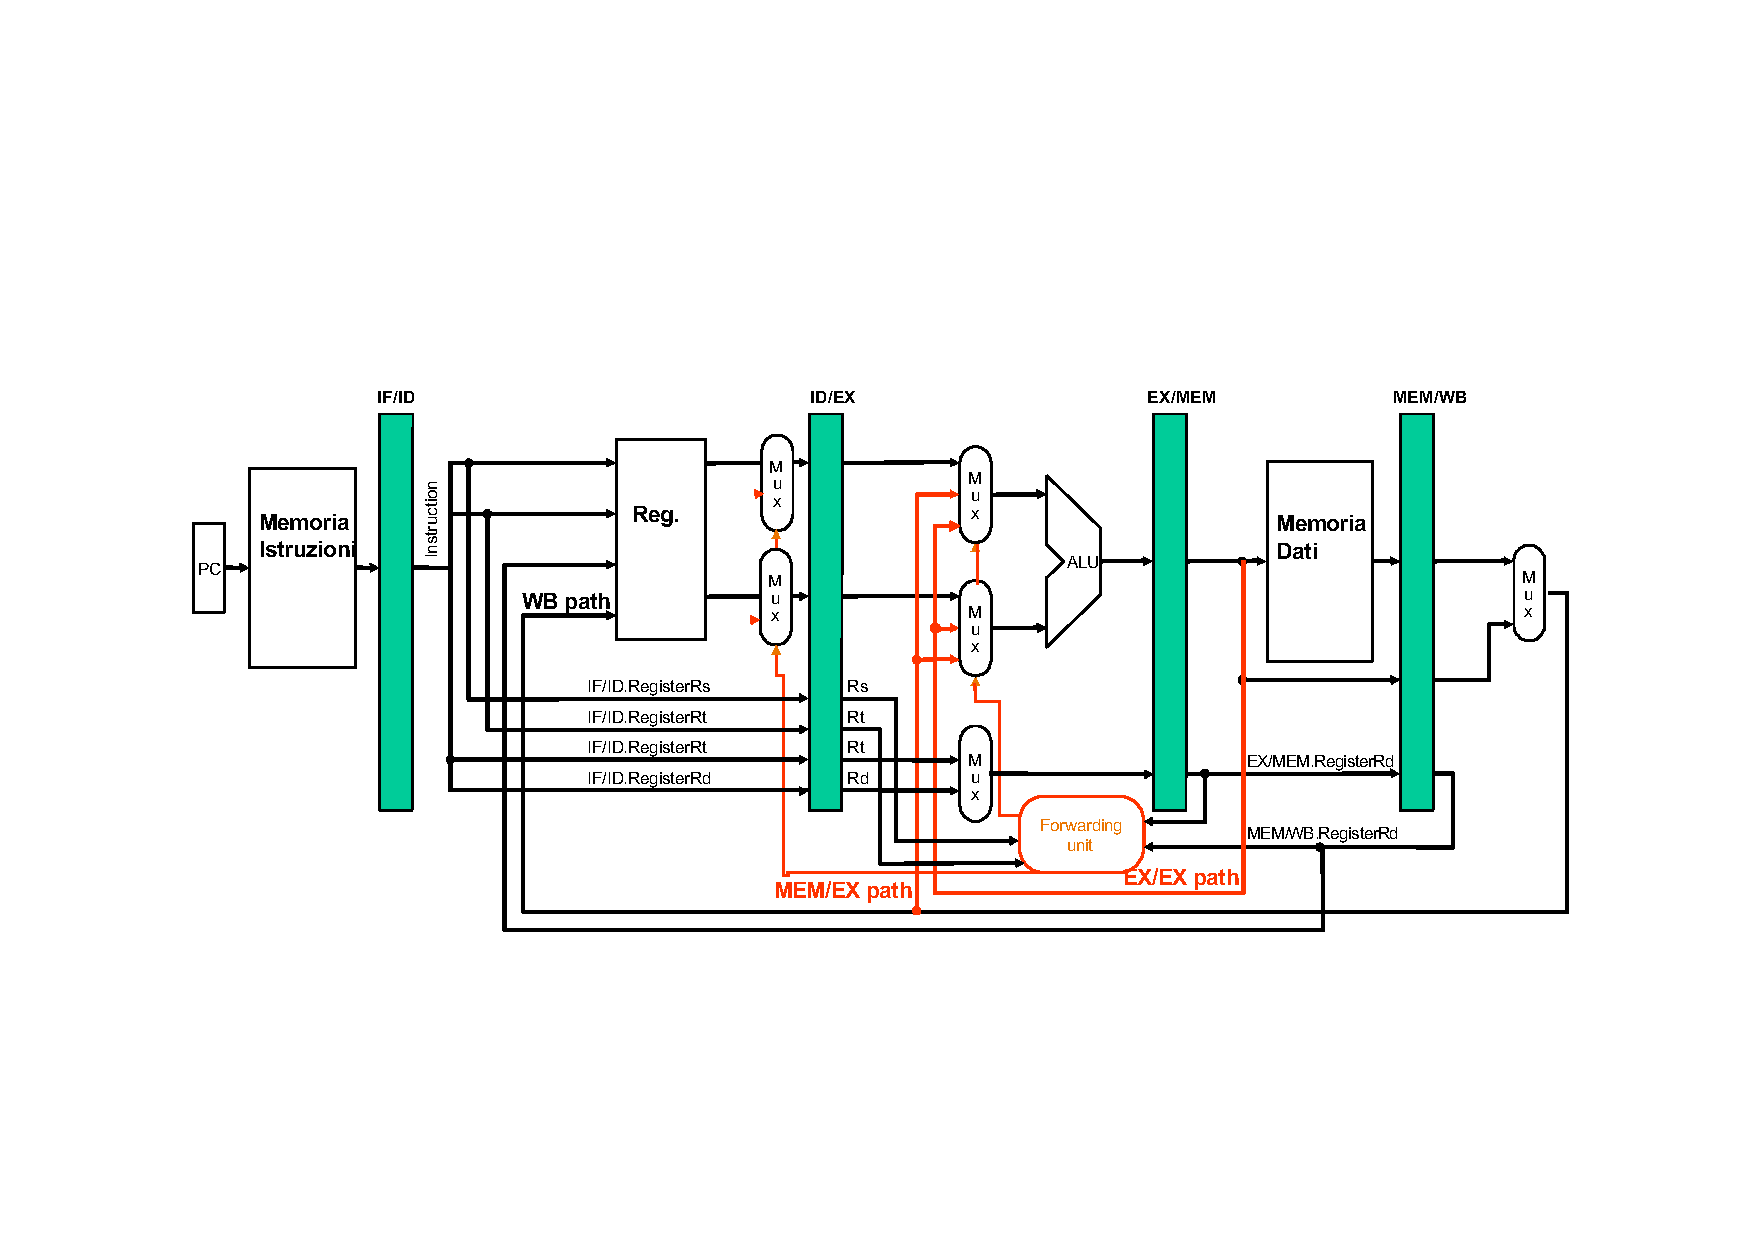
\includegraphics[width=\textwidth]{img/implementation-mips-forwarding-unit-1.pdf}
    \caption{Implementation of MIPS with \indexdefinition{Forwarding Unit}.\cite{pipelining-slides}}
    \label{fig: implementation of MIPS with Forwarding Unit}
\end{figure}

\noindent
Scan (or click) the QR code below to view the figure~\ref{fig: implementation of MIPS with Forwarding Unit} in high quality:
\begin{center}
    \qrcode{https://github.com/PoliMI-HPC-E-notes-projects-AndreVale69/HPC-E-PoliMI-university-notes/tree/main/advanced-computer-architectures/notes/img/implementation-mips-forwarding-unit-1.pdf}
\end{center}

\noindent
The forwarding paths created inside the MIPS architecture are three: \textbf{\texttt{EX} to \texttt{EX}} path, \textbf{\texttt{MEM} to \texttt{EX}} path, and \textbf{\texttt{MEM} to \texttt{MEM}} path.
\begin{figure}[!htp]
    \centering
    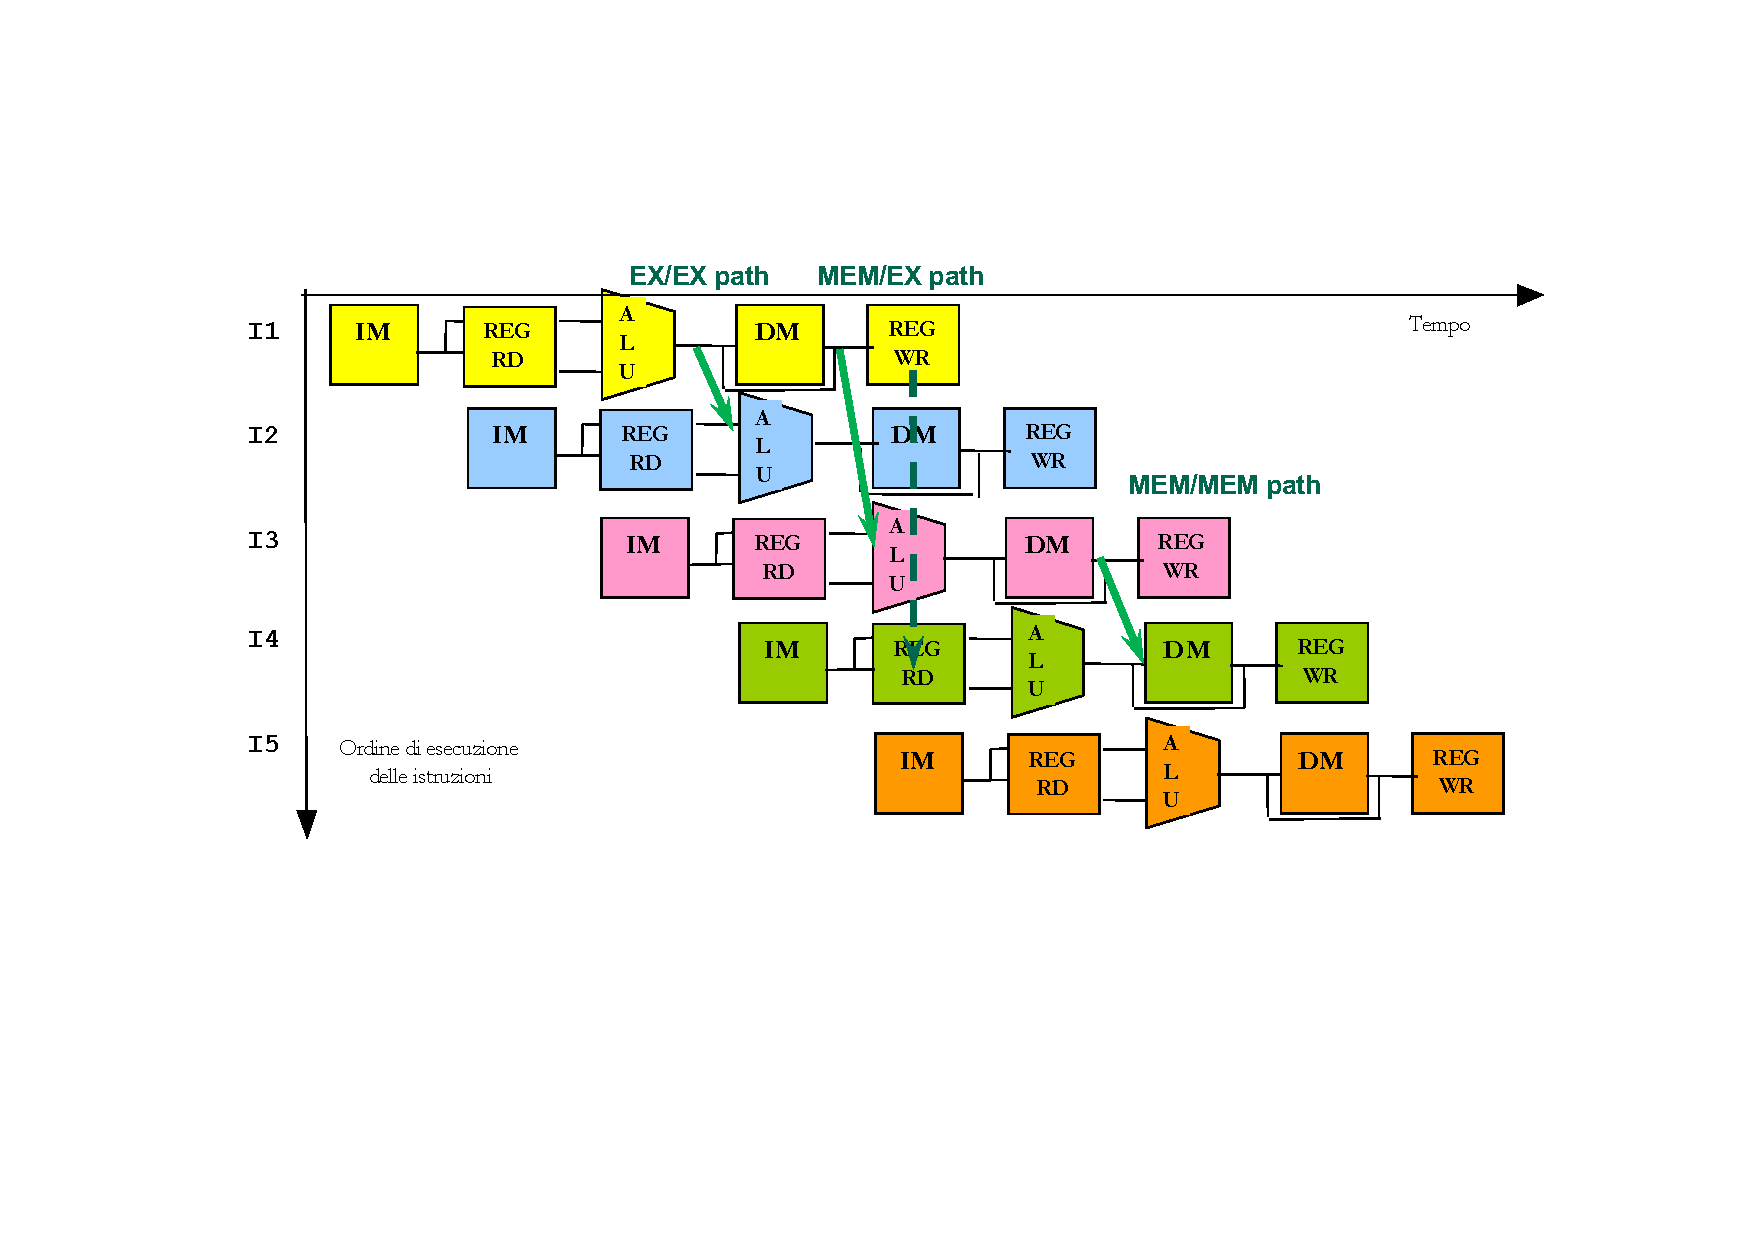
\includegraphics[width=\textwidth]{img/forwarding-paths-1.pdf}
    \caption{Forwarding paths on MIPS architecture.\cite{pipelining-slides}}
\end{figure}

\noindent
Furthermore, the \textbf{forwarding technique can solve} the \textbf{Load-Use} and \textbf{Load-Store} Data Hazard. It's a very interesting feature because the \texttt{MEM} to \texttt{EX} and \texttt{MEM} to \texttt{MEM} paths can solve two different situations:
\begin{itemize}
    \item \textbf{Load-Use} Hazard. It's \textbf{solved by MEM to EX path} because the value loaded in the MEM stage, is forwarded directly to the EX stage of the next conflict instruction (but unfortunately we need one stall to delay the run).

    \begin{examplebox}
        Given the following code:
        \lstinputlisting[language=misc]{code/solution-of-data-hazards/load-use-hazard-1.s}
        The \texttt{s0} operand depends on the load (\texttt{lw}) operator. Here, the problem of \textbf{\emph{load-use hazard}} occurs.
        \begin{center}
            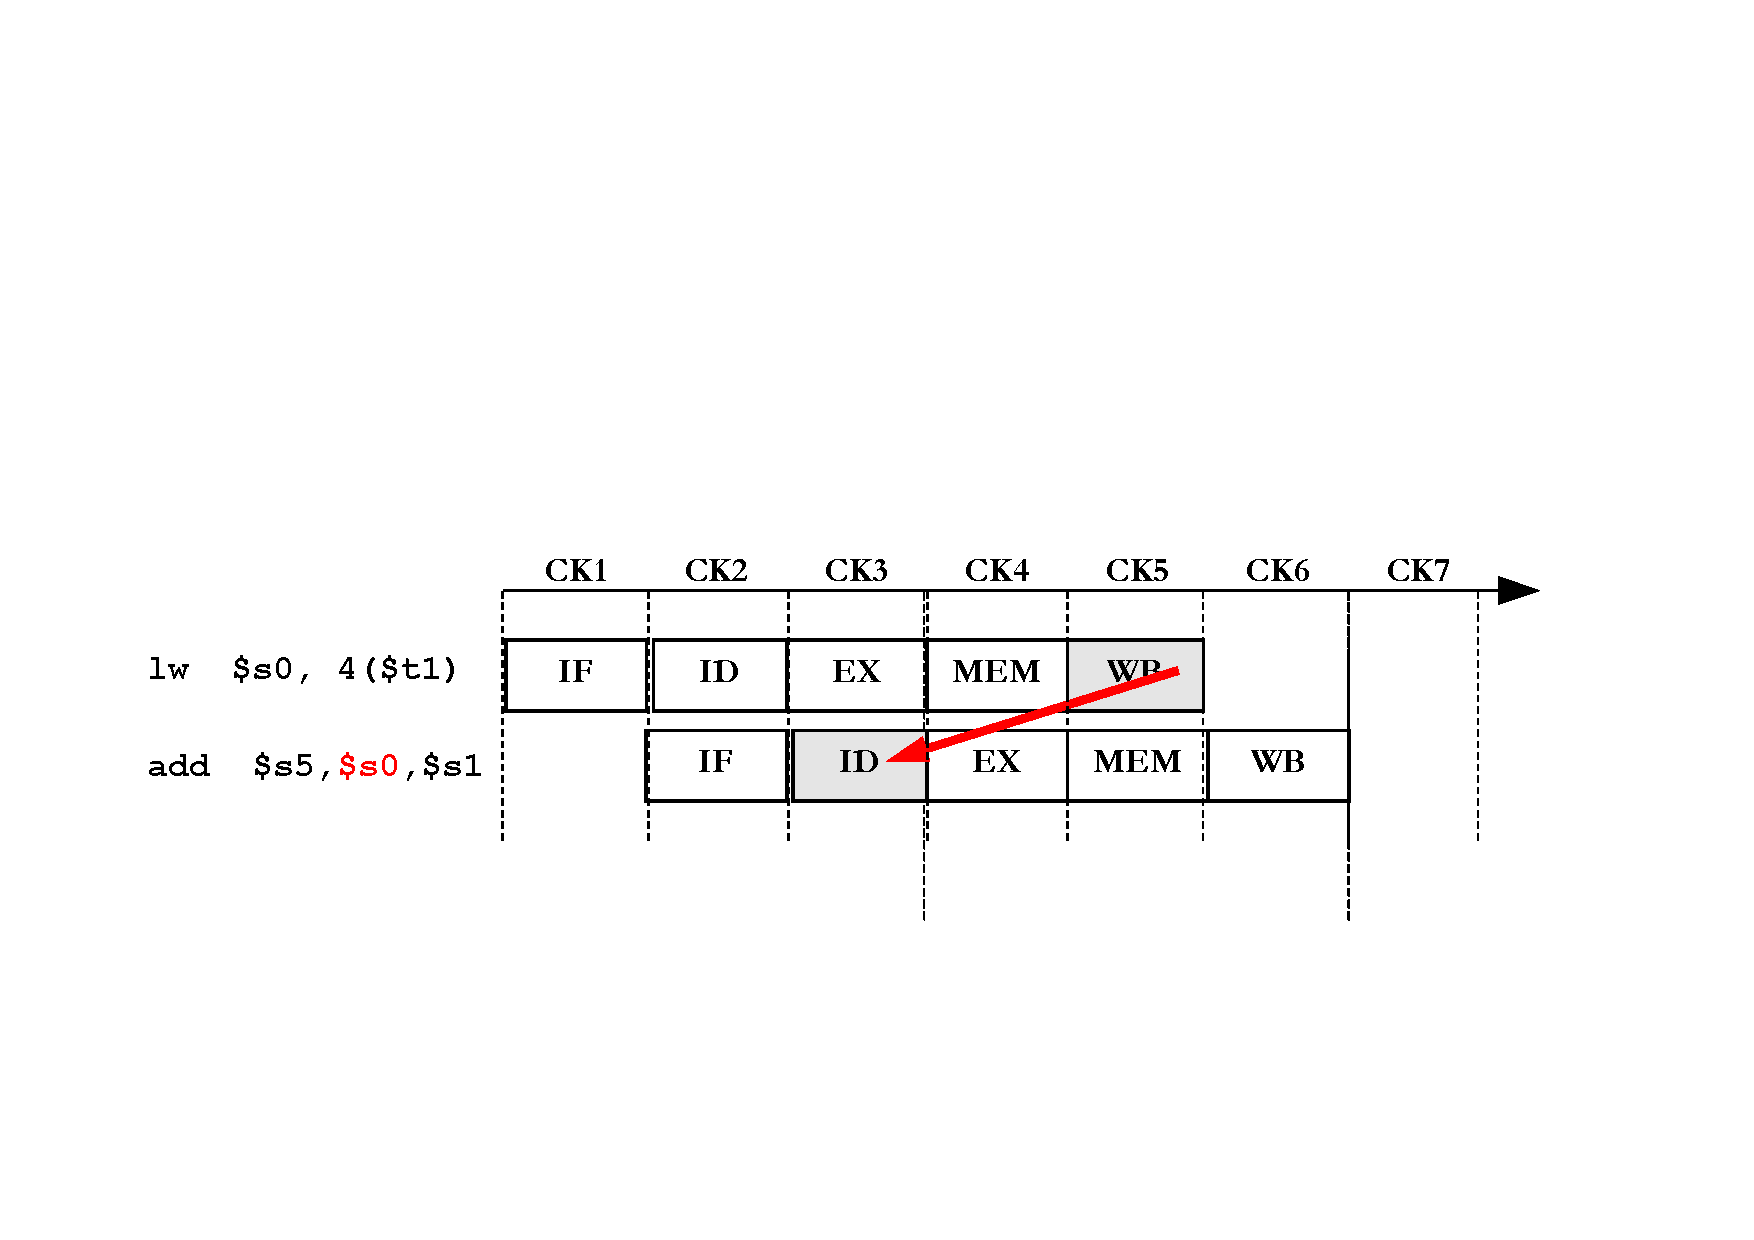
\includegraphics[width=\textwidth]{img/load-use-hazard-problem-1.pdf}
            \captionof*{figure}{The load-use hazard problem.\cite{pipelining-slides}}
        \end{center}
        In the figure, we can see the existing dependence. An ideal solution to the load-use hazard should be taking the value after the Memory Access operation (because the load instruction reads the effective address on the memory) and using it in the sum (operation).

        The \textbf{forwarding technique solves it using the MEM-EX path but using \underline{one stall}}.
        \begin{center}
            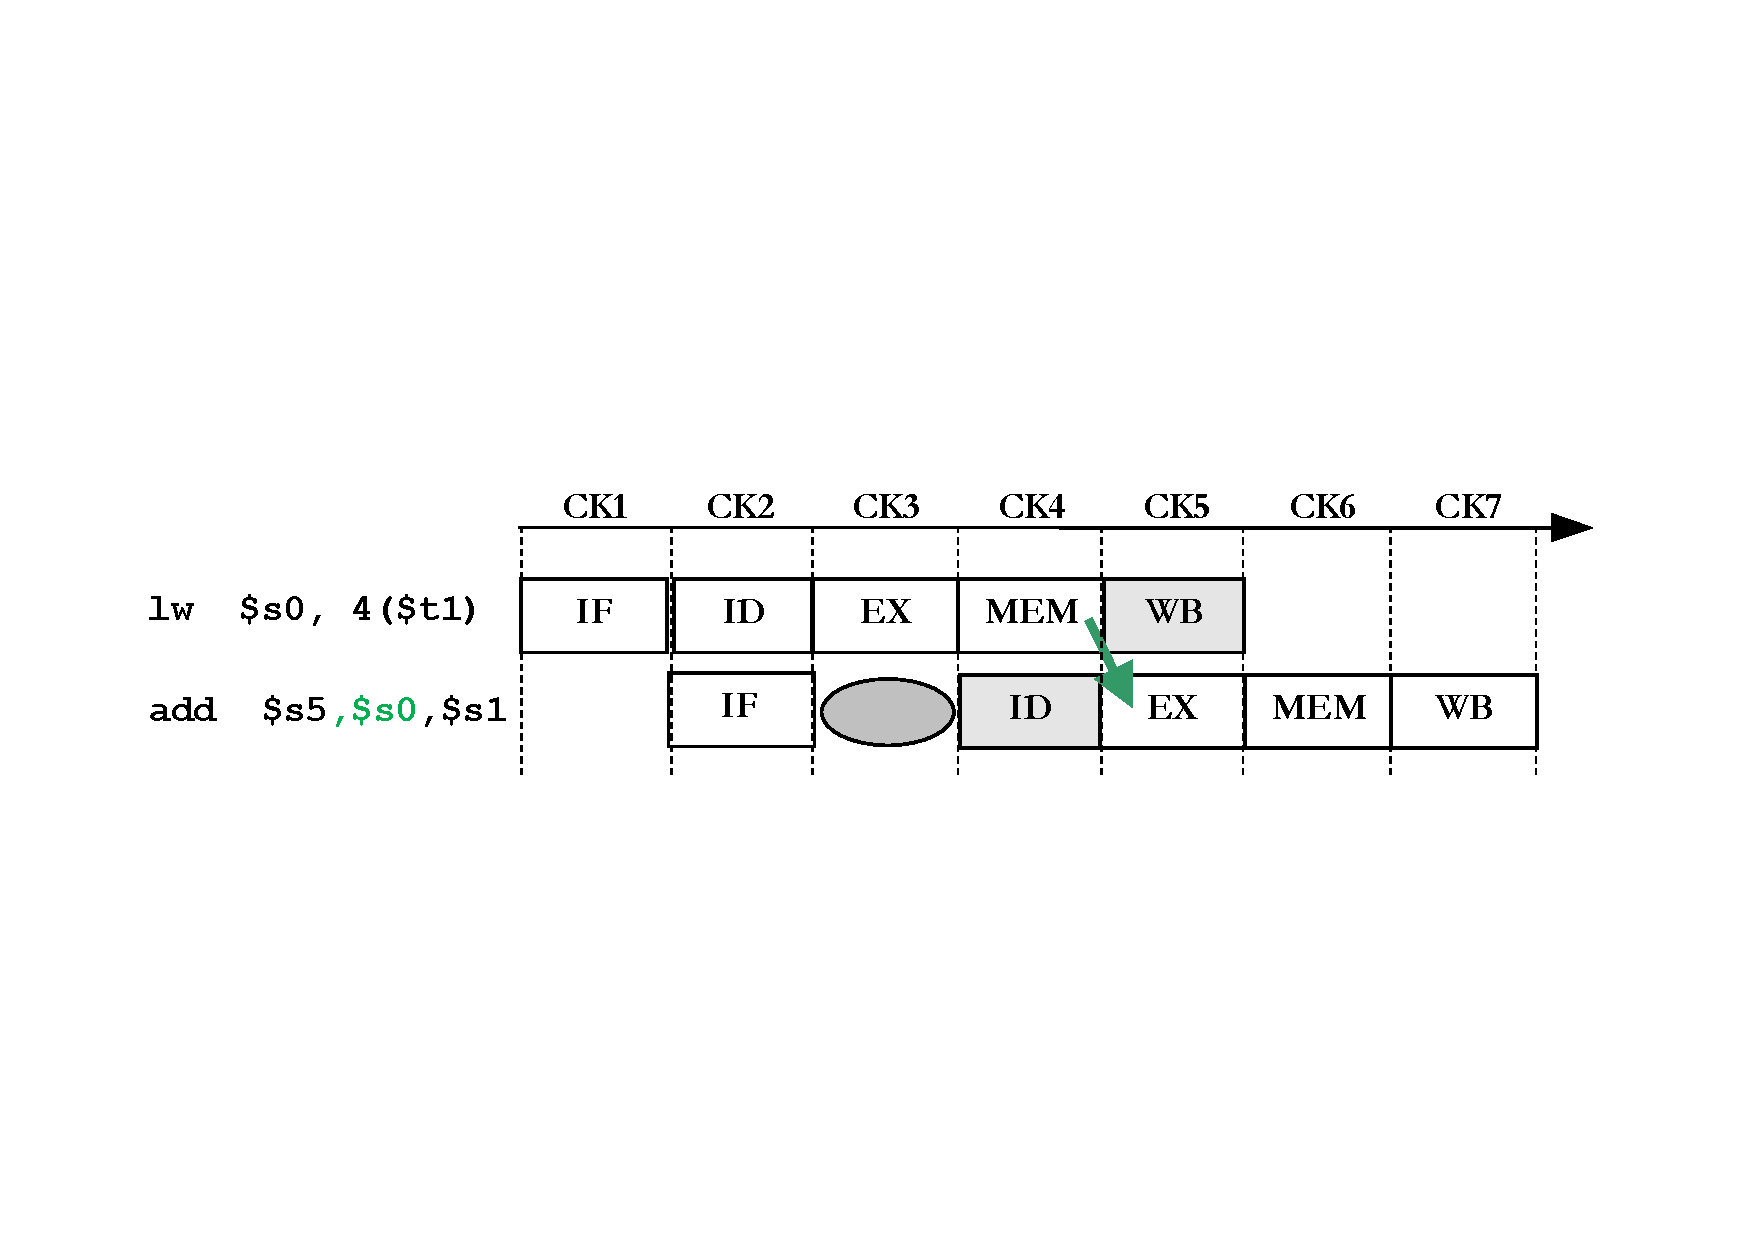
\includegraphics[width=\textwidth]{img/load-use-hazard-problem-2.pdf}
            \captionof*{figure}{Forwarding technique with MEM-EX path.\cite{pipelining-slides}}
        \end{center}
    \end{examplebox}

    \item \textbf{Load-Store} Hazard. It's \textbf{solved by MEM to MEM path} because the value loaded in the MEM stage, is forwarded directly to the MEM stage of the next conflict instruction.
    \begin{examplebox}
        Given the following code:
        \lstinputlisting[language=misc]{code/solution-of-data-hazards/load-store-hazard-1.s}
        The \texttt{s0} operand depends on the load (\texttt{lw}) operator. Here, the problem of \textbf{\emph{load-store hazard}} occurs.
        \begin{center}
            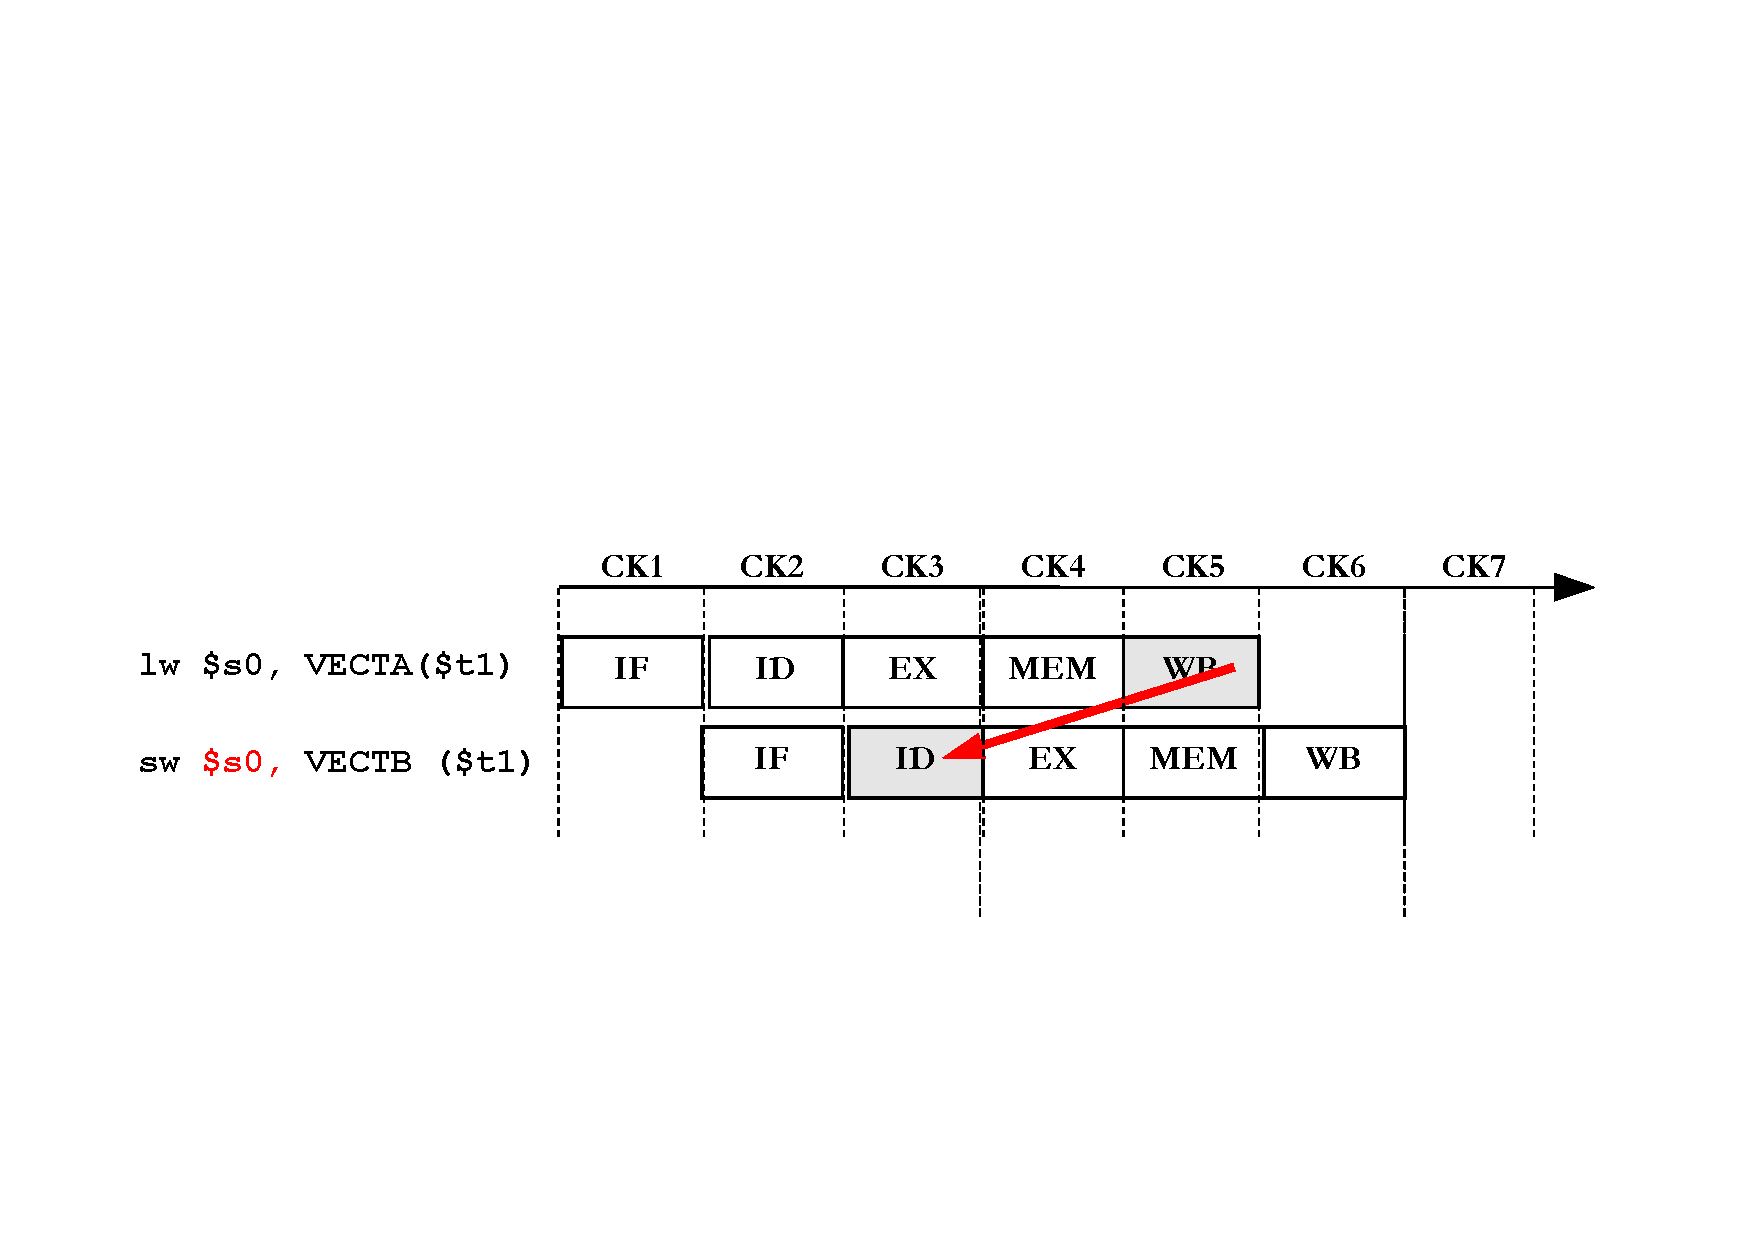
\includegraphics[width=\textwidth]{img/load-store-hazard-problem-1.pdf}
            \captionof*{figure}{The load-store hazard problem.\cite{pipelining-slides}}
        \end{center}
        In the figure, we can see the existing dependence. An ideal solution to the load-store hazard should be taking the value after the Write Back operation (because the load instruction writes the data read from memory in the destination register of the Register File) and using it in the Instruction Decode (because the ID includes also Register Read, then it reads from the Register File (RF)).

        The \textbf{forwarding technique solves it using the MEM-MEM path \underline{without any stall}}.
        \begin{center}
            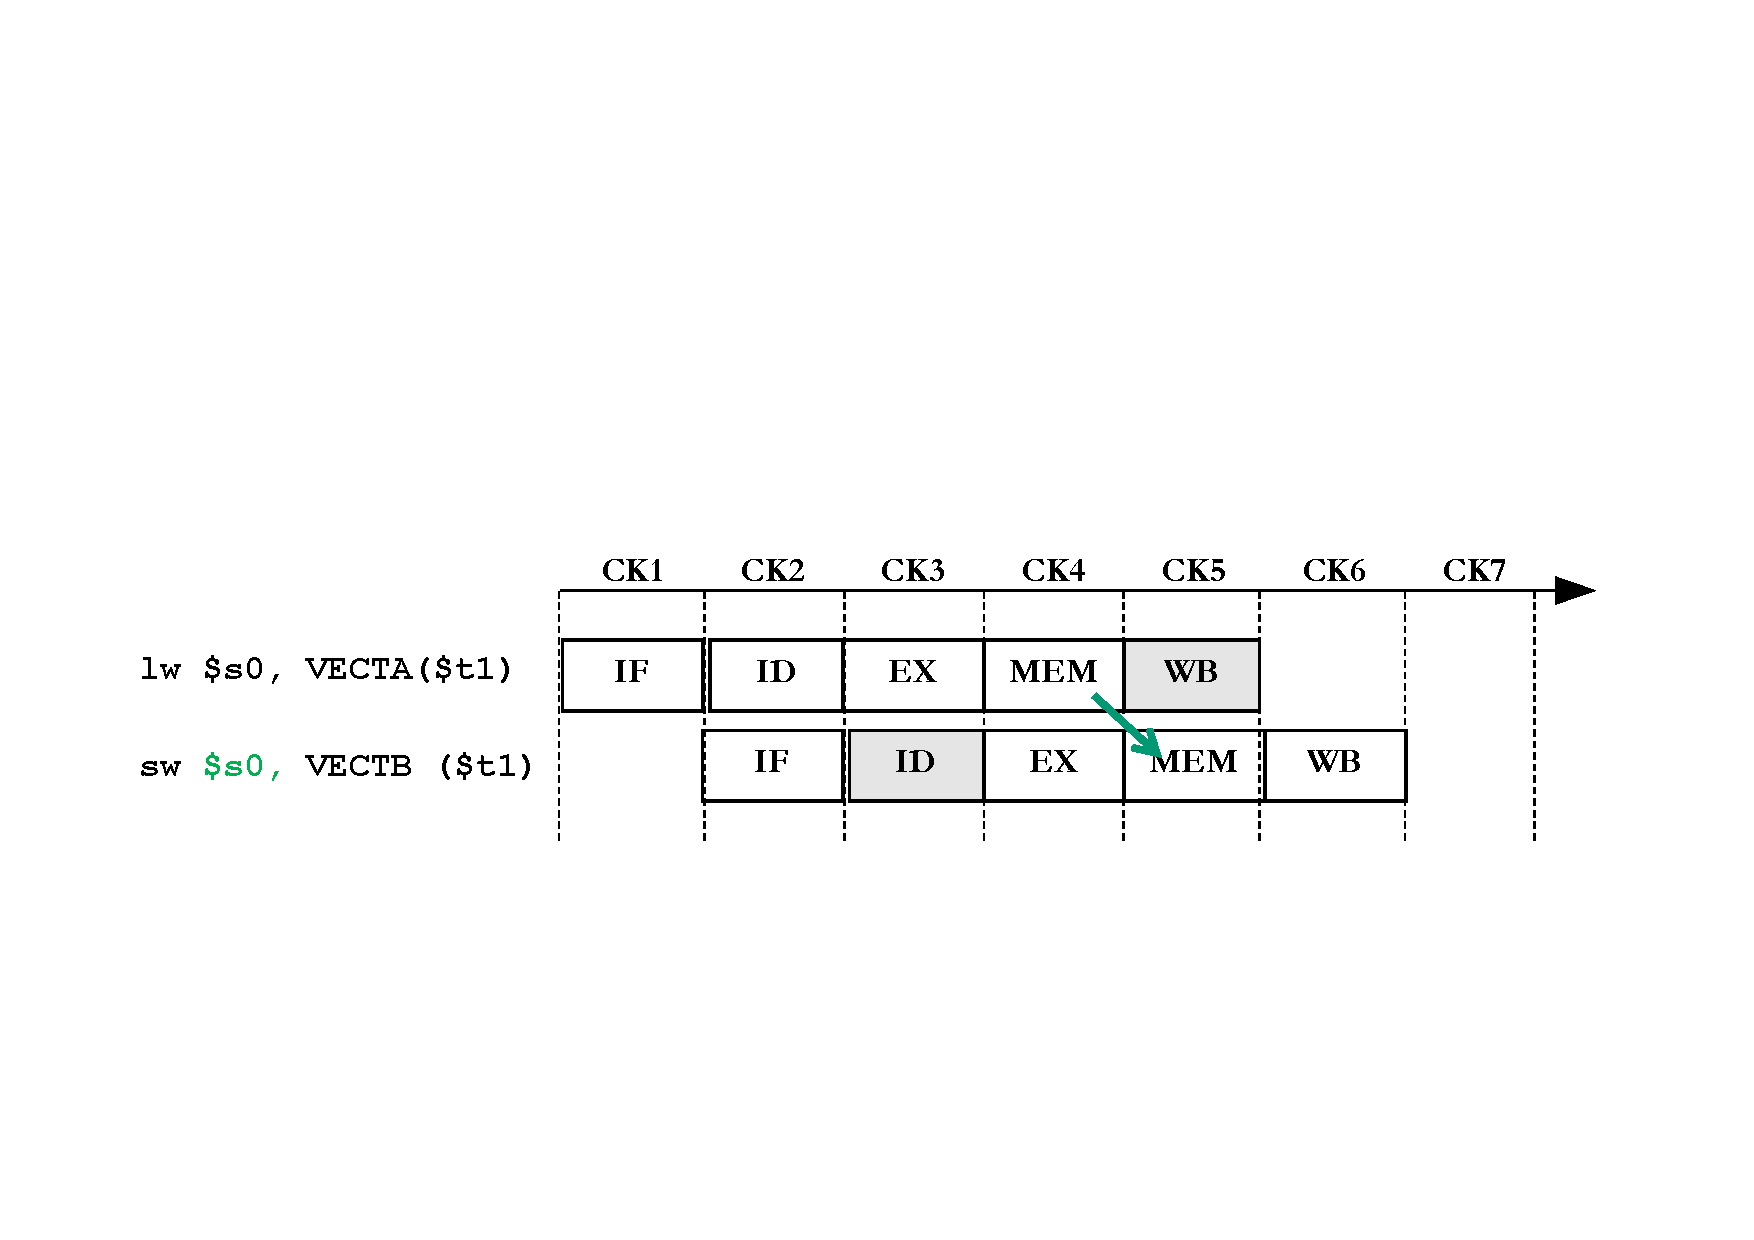
\includegraphics[width=\textwidth]{img/load-store-hazard-problem-2.pdf}
            \captionof*{figure}{Forwarding technique with MEM-MEM path.\cite{pipelining-slides}}
        \end{center}
    \end{examplebox}
\end{itemize}

\begin{examplebox}\label{example: insertion of nop}
    In the following figure, we can see how a \textbf{compilation technique}, the \textbf{insertion of \texttt{nop}}, can be solve the data hazard problem.
    \begin{center}
        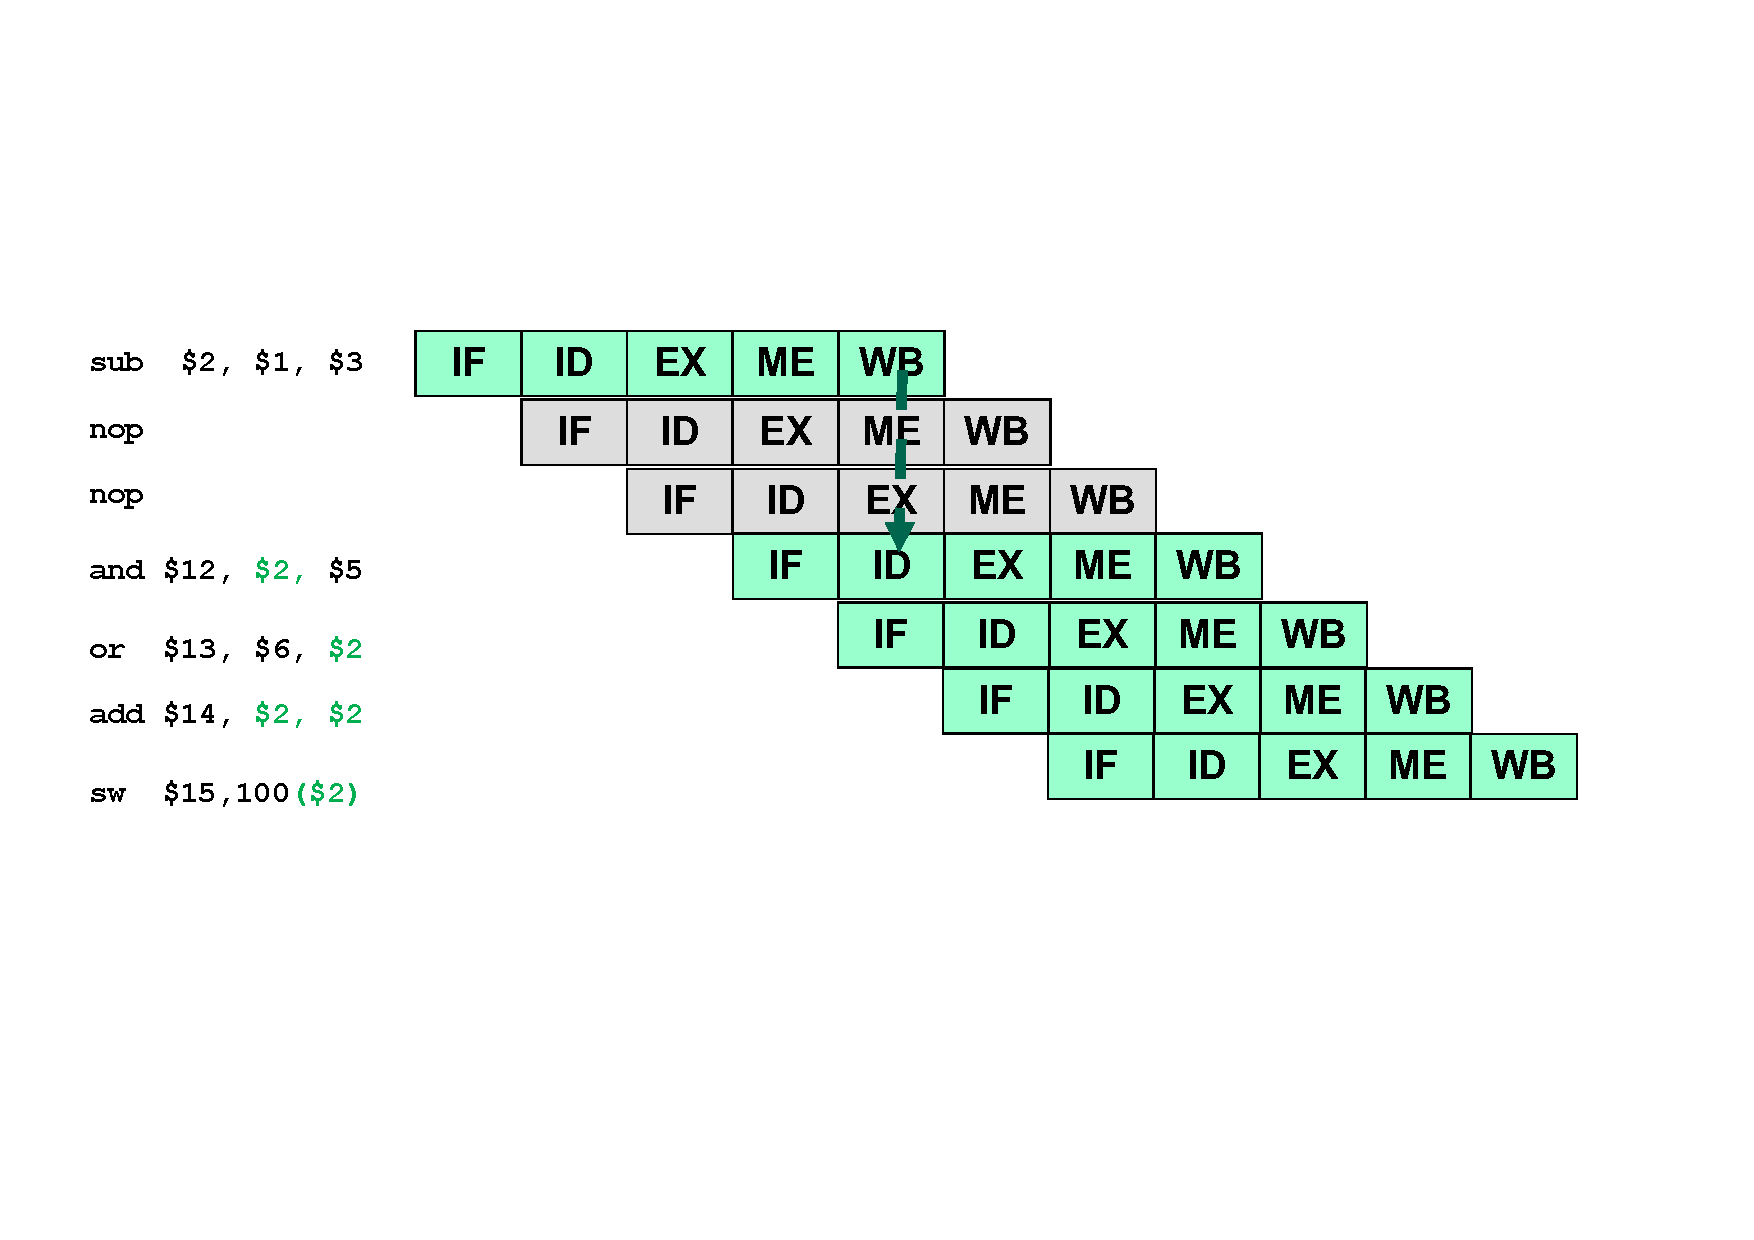
\includegraphics[width=\textwidth]{img/insertion-of-nop-1.pdf}
        \captionof*{figure}{Insertion of \texttt{nop}.\cite{pipelining-slides}}
    \end{center}
\end{examplebox}

\newpage

\begin{examplebox}\label{example: instructions scheduling}
    In the following figure, we can see how a \textbf{compilation technique}, the \textbf{instructions scheduling}, can be solve the data hazard problem.
    \begin{center}
        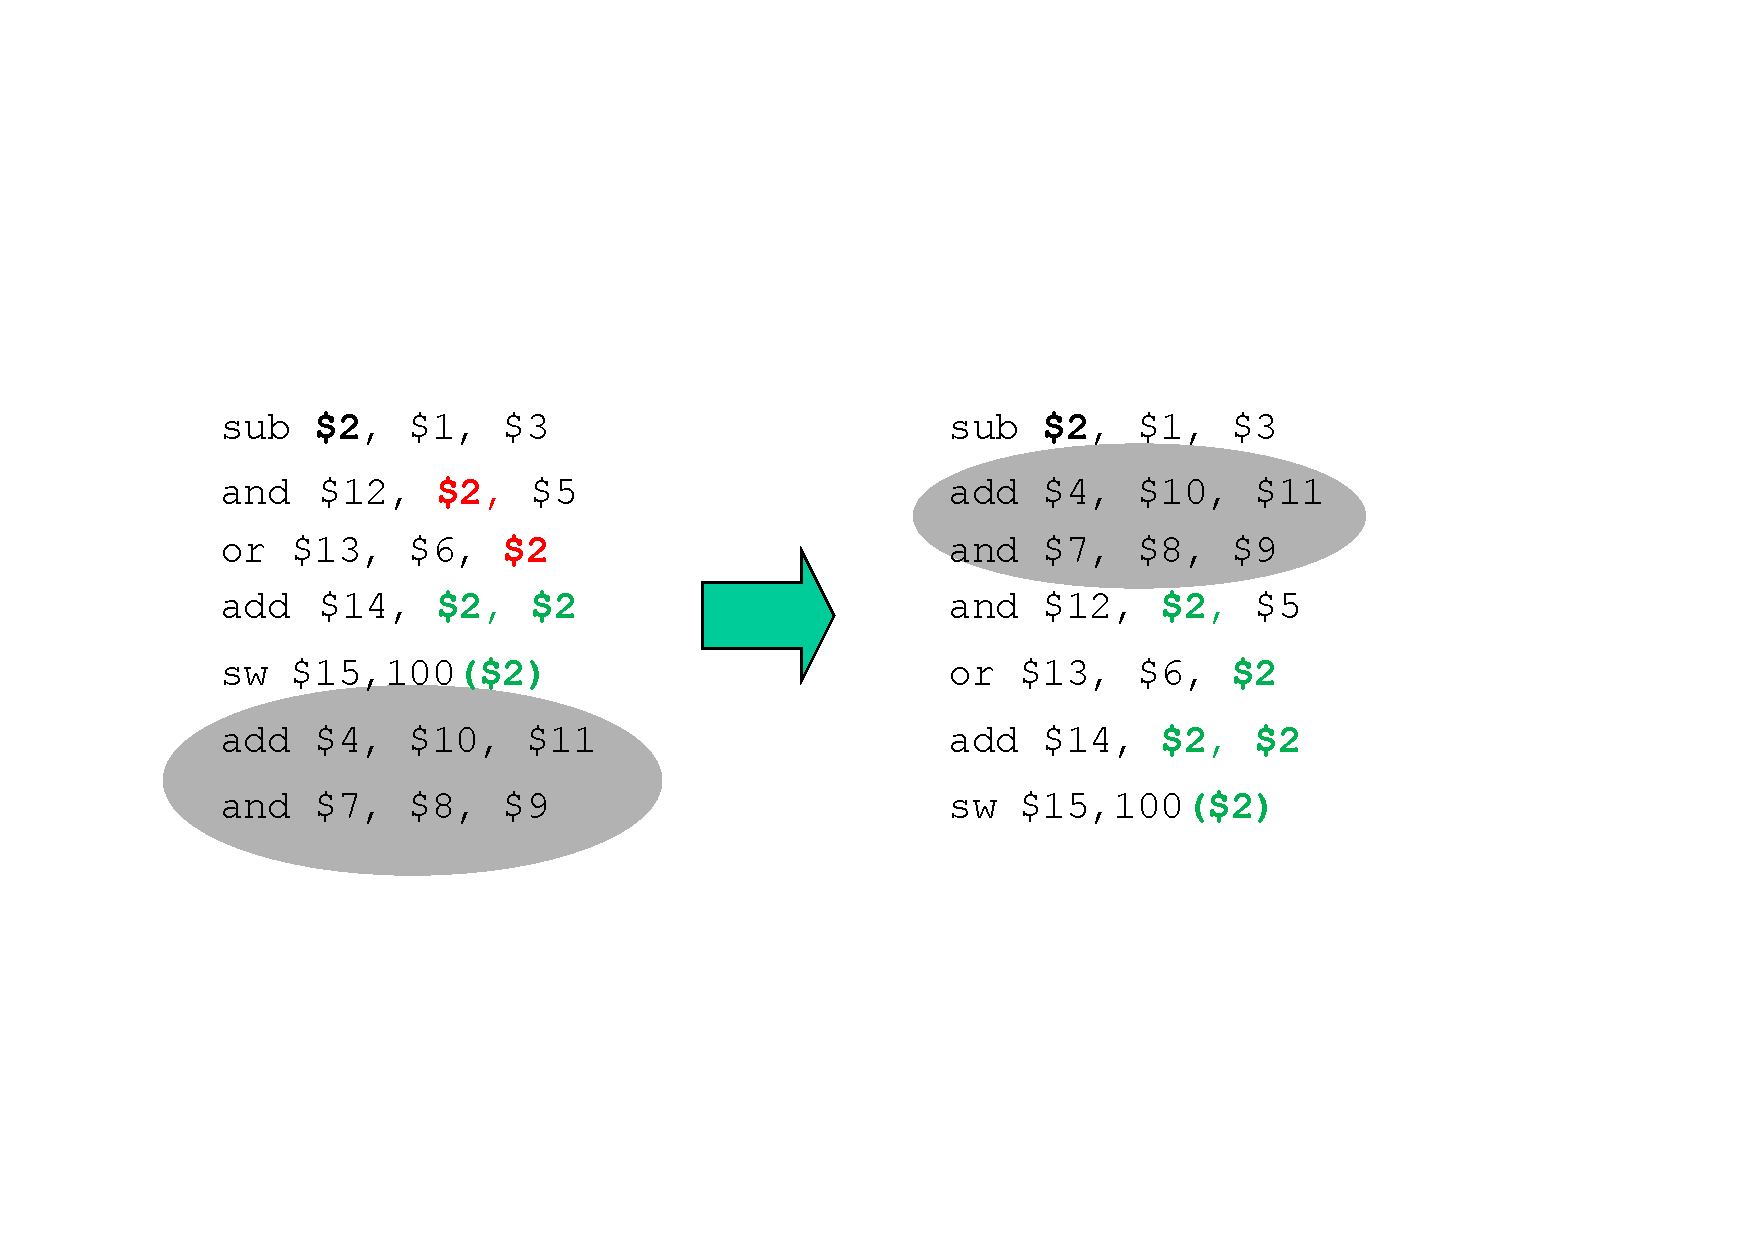
\includegraphics[width=\textwidth]{img/instructions-scheduling-1.pdf}
        \captionof*{figure}{Instructions scheduling.\cite{pipelining-slides}}
    \end{center}
\end{examplebox}

\begin{examplebox}\label{example: insertion of stalls}
    In the following figure, we can see how a \textbf{hardware technique}, the \textbf{insertion of stalls}, can be solve the data hazard problem.
    \begin{center}
        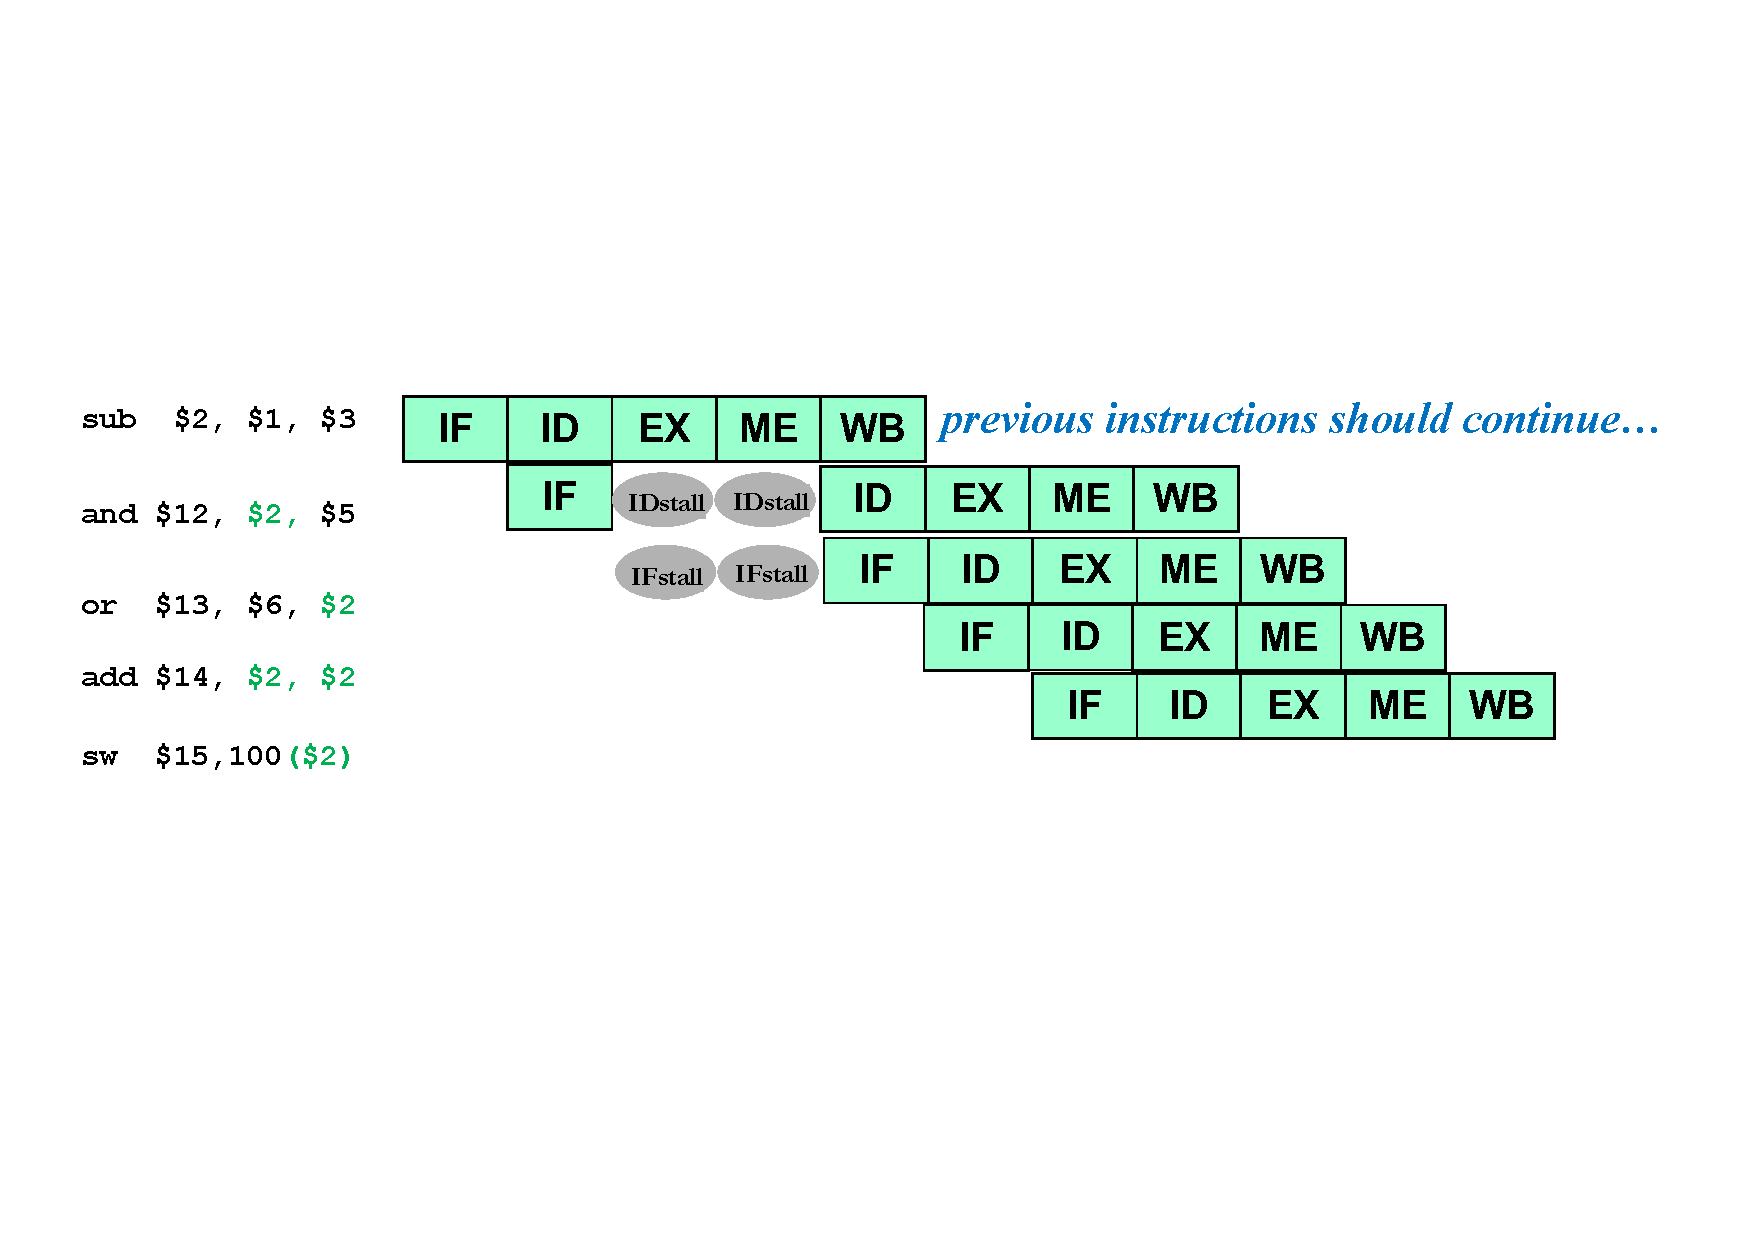
\includegraphics[width=\textwidth]{img/insertion-of-stalls-1.pdf}
        \captionof*{figure}{Insertion of stalls.\cite{pipelining-slides}}
    \end{center}
\end{examplebox}

\begin{examplebox}\label{example: data forwarding}
    In the following figure, we can see how a \textbf{hardware technique}, the \textbf{data forwarding}, can be solve the data hazard problem.
    \begin{center}
        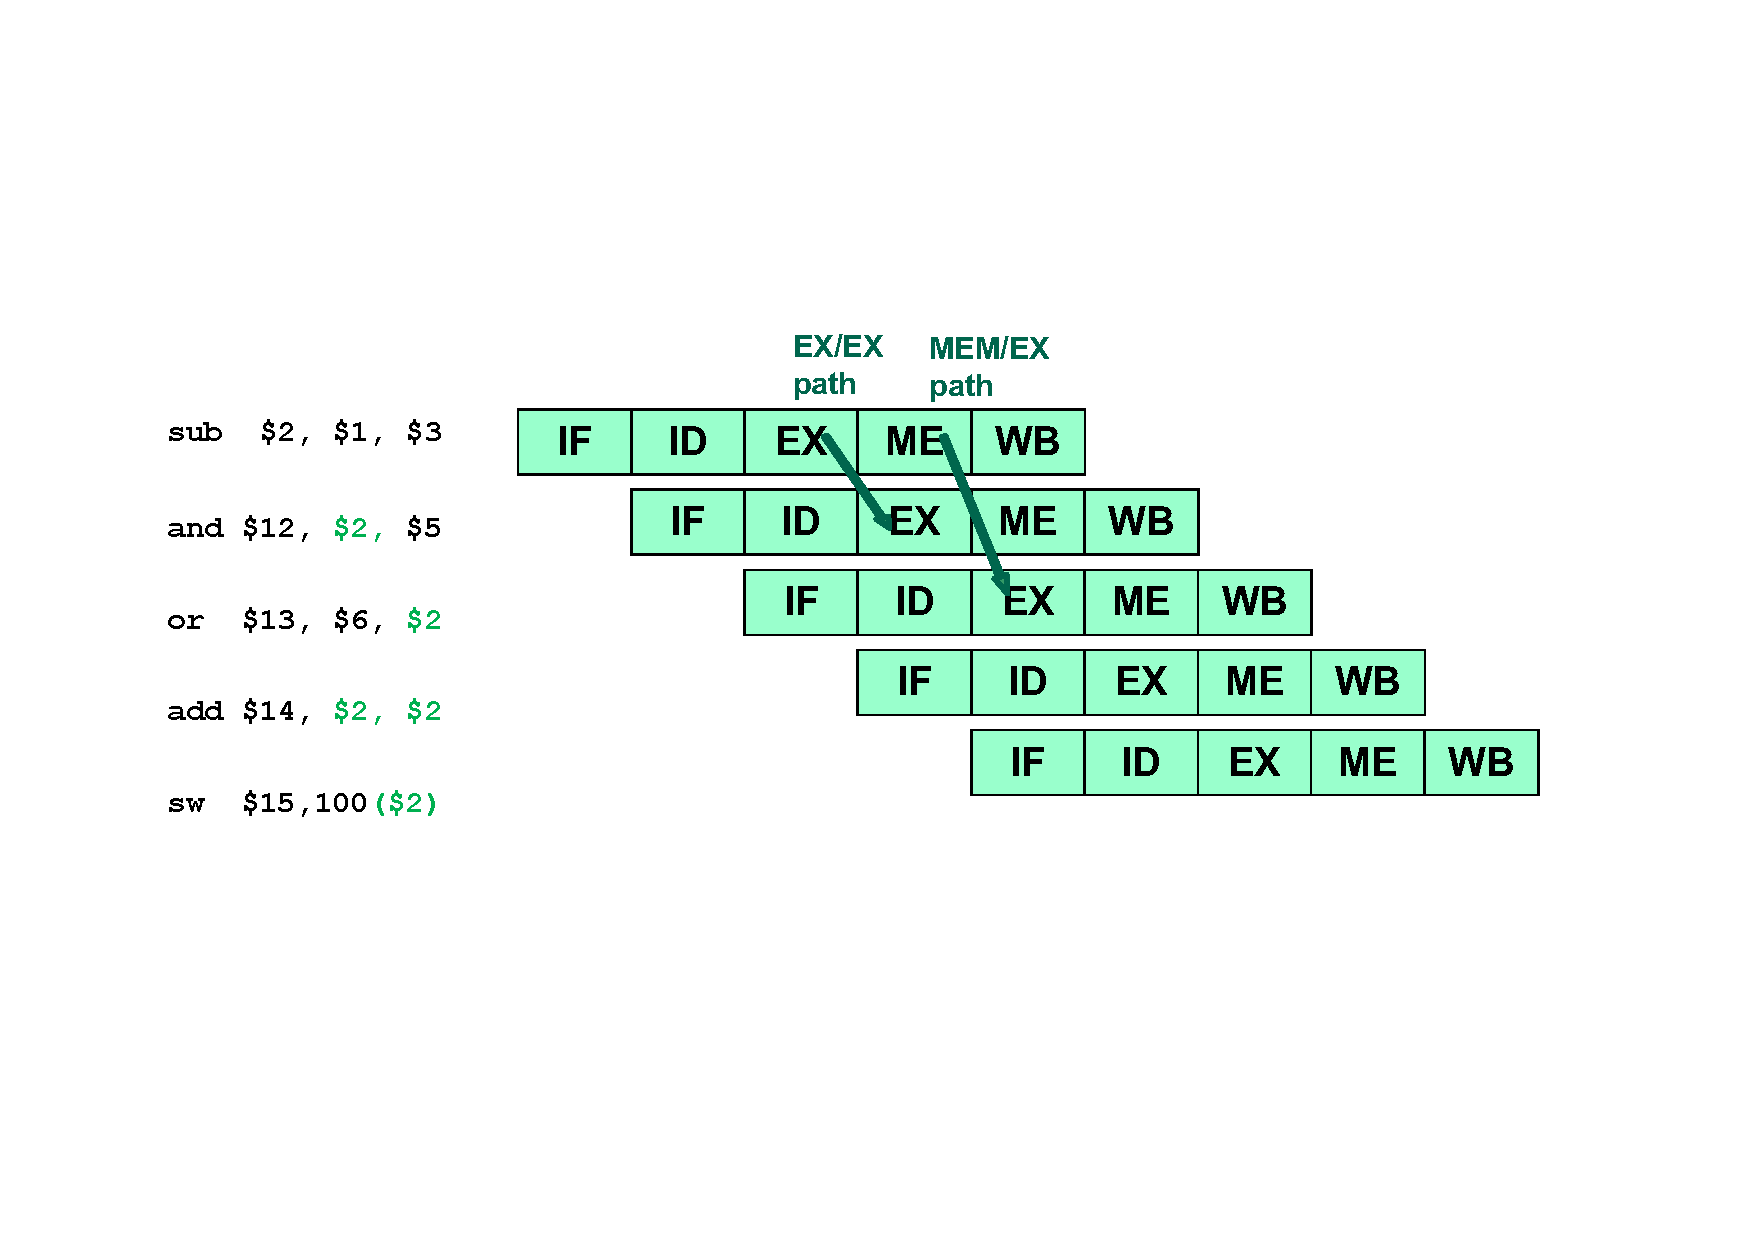
\includegraphics[width=\textwidth]{img/data-forwarding-1.pdf}
        \captionof*{figure}{Data forwarding.\cite{pipelining-slides}}
    \end{center}
\end{examplebox}